\subsection{Cosmology as resolution flow (self-contained interface extension)}
\label{app:cosmology_resolution_flow}

This appendix records a minimal cosmology interface in the same protocol language used throughout this paper.
The central idea is that changing resolution parameters $(m,n)$ is a physical operation (a protocol flow step), and the growth laws of the stable sector $|X_m|=F_{m+2}$ and of the mean degeneracy $2^m/|X_m|$ provide a quantitative capacity-growth backbone.

\subsubsection{Initialization: the big bang as resolution bootstrapping}
\label{subsec:cosmo_init}

\InterfaceTag In a readout cosmology, the ``big bang'' is interpreted as resolution initialization of the readout hardware:
the system starts at small window length $m$ and small addressing order $n$, and rapidly enters a regime where nontrivial stable types exist and can be maintained under projection.
The balanced interface $m=2n$ provides a minimal coupling between a spatial grid and a local readout alphabet, and the anchor $(m,n)=(6,3)$ supplies the smallest fully explicit computable layer with nontrivial folding $64\to 21$.

\subsubsection{Inflation as exponential growth of stable capacity}
\label{subsec:cosmo_inflation_capacity}

As window length increases by $\Delta m$, the stable type count grows as
\[
|X_m|=F_{m+2}\sim \frac{\varphi^{m+2}}{\sqrt{5}},
\]
so stable capacity grows exponentially in $m$.
If an early epoch has approximately linear resolution growth $m(t)\approx m_0+\alpha t$, then
\[
|X_{m(t)}|\asymp \varphi^{m(t)}\asymp \e^{(\alpha\log\varphi)\,t},
\]
which provides a purely combinatorial capacity-growth analogue of an inflationary exponential stage (no additional inflaton field is introduced at the protocol level).

\subsubsection{Hidden-sector dominance at high resolution}
\label{subsec:cosmo_hidden_fraction}

The folding map compresses $2^m$ microstates into $F_{m+2}$ stable types.
Define the stable fraction and hidden fraction at window length $m$ by
\[
f_{\mathrm{stab}}(m):=\frac{|X_m|}{|\Omega_m|}=\frac{F_{m+2}}{2^m},
\qquad
f_{\mathrm{hid}}(m):=1-f_{\mathrm{stab}}(m),
\]
and the mean degeneracy
\[
d_m:=\frac{|\Omega_m|}{|X_m|}=\frac{2^m}{F_{m+2}}.
\]
Since $F_{m+2}\asymp \varphi^m$ and $\varphi<2$, one has $f_{\mathrm{stab}}(m)\to 0$ and $f_{\mathrm{hid}}(m)\to 1$ as $m\to\infty$; equivalently $d_m\asymp (2/\varphi)^m$ grows exponentially.

\subsubsection{A discrete energy-budget fit (interface hypothesis)}
\label{subsec:cosmo_energy_budget_fit}

\begin{assumption}[Readout-occupancy energy accounting (interface)]
\label{ass:occupancy_energy_z128}
Fix an effective window length $m$.
Assume that, on sufficiently coarse scales, the fractional contribution of a sector to the cosmic energy budget is proportional to long-time occupancy of the corresponding readout microstate subset.
Under a maximal-ignorance approximation at fixed resolution, this occupancy is approximated by counting measure on $\Omega_m$ (maximum-entropy/maximum-ignorance rationale; see, e.g., \cite{Jaynes1957,CoverThomas2006}), so that
\[
\Omega_{\mathrm{vis},0}\approx f_{\mathrm{stab}}(m),
\qquad
\Omega_{\mathrm{dark},0}\approx f_{\mathrm{hid}}(m)=1-f_{\mathrm{stab}}(m).
\]
\end{assumption}

\InterfaceTag Given a target present-day visible fraction $\Omega_{\mathrm{vis},0}$ (e.g.\ baryon fraction as a minimal proxy), Assumption~\ref{ass:occupancy_energy_z128} selects an effective integer window length $m_\ast$ by discrete matching.
Because $f_{\mathrm{stab}}(m)$ is strictly decreasing in $m$, this selection is unique once a target is fixed.
\MatchTag Using the Planck-2018 baryon fraction $\Omega_{\mathrm{b},0}\approx 0.0493$ as a compact target \cite{Planck2018Parameters}, the discrete match is
\[
\frac{F_{17}}{2^{15}}=\frac{1597}{32768}\approx 0.0487,%
\]
\MatchTag Selected $m_\ast=15$, $f_\mathrm{stab}(m_\ast)=4.873657\times 10^{-2}$, $f_\mathrm{hid}/f_\mathrm{stab}=1.951847\times 10^{1}$, with $(\Omega_\mathrm{hid}/\Omega_\mathrm{vis})_\mathrm{ref}=(1-\Omega_{\mathrm{vis},0})/\Omega_{\mathrm{vis},0}=1.928398\times 10^{1}$, $\log\!\bigl((f_\mathrm{hid}/f_\mathrm{stab})/(\Omega_\mathrm{hid}/\Omega_\mathrm{vis})_\mathrm{ref}\bigr)=1.208683\times 10^{-2}$.
Optional DM-only comparison (matching-layer): $(\Omega_\mathrm{DM}/\Omega_\mathrm{b})_\mathrm{ref}=5.360000$, $\log\!\bigl((f_\mathrm{hid}/f_\mathrm{stab})/(\Omega_\mathrm{DM}/\Omega_\mathrm{b})_\mathrm{ref}\bigr)=1.292397$.
\AuditTag Stability diagnostic: for $\Omega_{\mathrm{vis},0}=0.049300\pm 0.000500$ (1$\sigma$), the admissible discrete set is $\{15\}$ (stable).
\InterfaceTag This suggests $m_\ast\approx 15$ as a minimal discrete fit point under the stated interface hypothesis.
Figure~\ref{fig:cosmology_energy_budget_fit} provides a direct visualization of the discrete matching curve.

\begin{figure}[t]
\centering
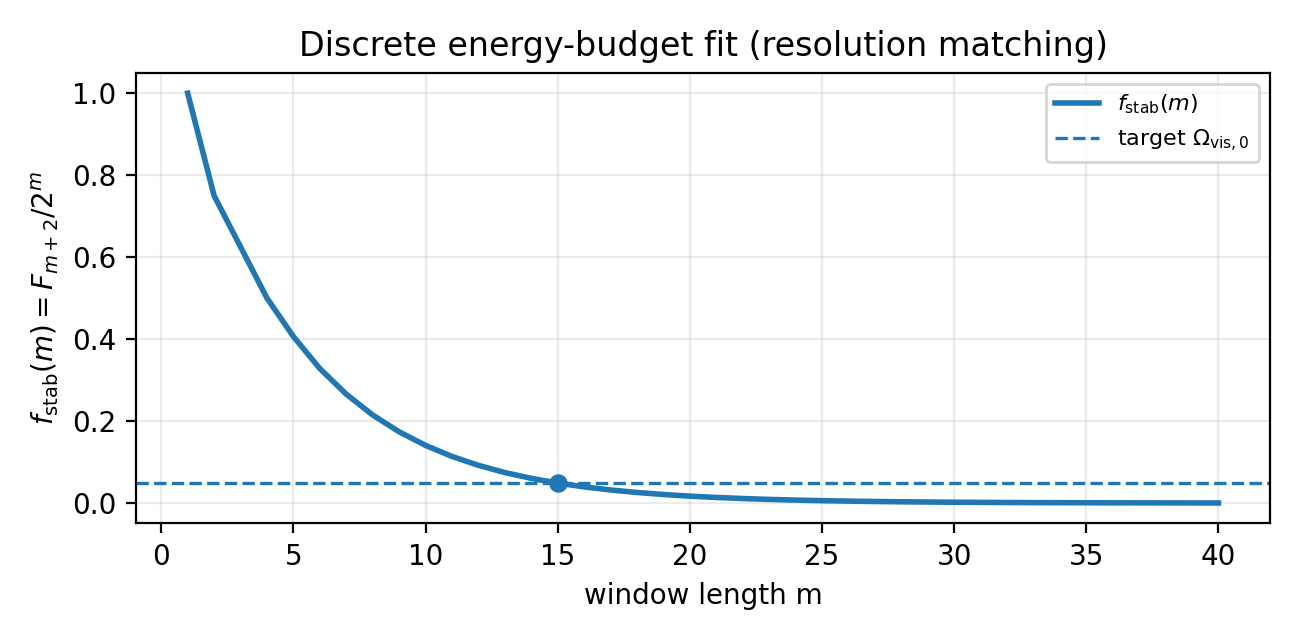
\includegraphics[width=0.85\linewidth]{figures/cosmology_energy_budget_fit.png}
\caption{Discrete matching curve for $f_{\mathrm{stab}}(m)=F_{m+2}/2^m$ against the target $\Omega_{\mathrm{vis},0}$ used in the text. The figure is generated by \texttt{scripts/exp\_cosmology\_energy\_budget\_fit.py}.}
\label{fig:cosmology_energy_budget_fit}
\end{figure}

\paragraph{Status and falsifiability.}
\AuditTag The assumption is explicitly flagged as an interface hypothesis.
Its falsifiability route is to compare the implied hidden/stable ratio $f_{\mathrm{hid}}(m_\ast)/f_{\mathrm{stab}}(m_\ast)=d_{m_\ast}-1$ with an observationally declared reference ratio.
\MatchTag Under the literal reading of Assumption~\ref{ass:occupancy_energy_z128} with $\Omega_{\mathrm{dark},0}=1-\Omega_{\mathrm{vis},0}$, the reference ratio is $(1-\Omega_{\mathrm{vis},0})/\Omega_{\mathrm{vis},0}$ (fixed once $\Omega_{\mathrm{vis},0}$ is chosen).
\MatchTag If instead one interprets ``dark'' as ``dark matter only'' while treating dark energy separately, one may compare to $\Omega_{\mathrm{DM}}/\Omega_{\mathrm{b}}$ (Planck-2018 baseline; \cite{Planck2018Parameters}), as reported in the generated summary for transparency.
Independently, one can test whether reconstructed overhead proxy fields (Section~\ref{app:chi_reconstruction_protocol}) show the predicted address-aware invariances and correlations under declared counterfactual baselines.

